Graph-relabeling-systems introduced in \cite{litovsky1999graph} are rewriting systems. For a given graph, a graph relabeling system identify a subgraph of the graph and modify the labels of the nodes and edges of this subgraph. Since it never modifies the structure of the graph, it is very intuitive.

% \begin{definition}[Graph Relabeling Rule]
%   A \emph{graph relabeling rule} is a couple of labeled graphs \( ((U,\lambda),(U, \lambda')) \) where \( (U, \lambda) \) is said to be the \emph{left-hand side graph} and \( (U, \lambda')\) the \emph{right-hand side graph}.
% \end{definition}  
\begin{definition}[Rule]
  \label{def:gls_rule}
  A \textbf{GLS rewriting rule} is an ordered pair of labeled graphs \( (U,\lambda) \to (U, \lambda') \) that share the same underlying unlabeled graph \( U \). The labeled graph \( (U, \lambda) \) is said to be the \textbf{left-hand side graph} and \( (U, \lambda')\) the \textbf{right-hand side graph}.
\end{definition} 
 
% \begin{definition}[Match]
%   Let \(((U,\lambda),(U, \lambda')) \) be a graph relabeling rule. A \emph{match} of this rule in a labeled graph \( (G, \lambda_G) \) is a graph homomorphism \( m : (U,\lambda) \to (G, \lambda_G) \).
% \end{definition}
\begin{definition}[Match]
  \label{def:gls_match}
  Let \( L \to R \) be a GLS rewriting rule and \( G \) a labeled graph.
  A \textbf{GLS match} of this rule in \( G \) is a monomorphism \( m : L \rightarrowtail G \).
\end{definition}

% \begin{definition}[Witness of a rewriting step]
%   \label{def:witness_rewriting_step}
%   Let \( \rho = ((U,\lambda),(U, \lambda')) \) be a graph relabeling rule.
%   A couple of labeled graph morphisms $(m : (U,\lambda_U) \rightarrowtail (G,\lambda_G), m': (U, \lambda_U') \rightarrowtail (G, \lambda'_G))$ that share the same underlying unlabeled graph homomorphism defines a rewriting step from $(G, \lambda_G)$ to $(G, \lambda'_G)$ using the rule $\rho$ and match $m$.
% \end{definition}
% \begin{definition}[Witness]
%   \label{def:gls_witness}
%   Let \( \rho = L \to R \) be a graph relabeling rule. Let \( (G, \lambda_G), (G, \lambda'_G) \) be a labeled graph.
%   Let \( m : L \to (G,\lambda_G) \) be a match of \( \rho \) in \( (G, \lambda_G) \).
%   A couple of labeled graph morphisms $(m, m': R \rightarrowtail (G, \lambda'_G))$ such that $m(x) = m'(x)$ for all nodes and edges $x$ in $G$ is witness a \textbf{graph relabeling step} from $(G, \lambda_G)$ to $(G, \lambda'_G)$ using the rule $\rho$ and match $m$, and we denote $(G,\lambda) \Rightarrow_{\rho,\mathfrak{gls}}^m (G,\lambda')$.
% \end{definition}

\begin{definition}[Witness of rewriting step and rewriting step]
  \label{def:gls_witness_rewriting_step}
  Let \( \rho = (L, \lambda_L) \to (R,\lambda_R) \) be a GLS rewriting rule, \( (G, \lambda_G) \) a labeled graph and \( m : (L, \lambda_L) \rightarrowtail (G,\lambda_G) \) a match of \( \rho \) in \( (G, \lambda_G) \).
  
  Let $\lambda'_G$ be a labeling function on the nodes and edges of \( G \) such that \( \lambda'_G(x) = \lambda_G(x) \) for all nodes and edges \( x \) in \( G \setminus \operatorname{Im}(m) \), and \( \lambda'_G(x) = \lambda_R(m^{-1}(x)) \) otherwise.

  Let $m' : (R, \lambda_R) \rightarrowtail (G, \lambda'_G)$ be a graph homomorphism such that \( m(x) = m'(x) \) for all nodes and edges \( x \) in \( G \).

  The ordered pair $(m, m')$ is a \textbf{witness} of the \textbf{rewriting step} from \( (G, \lambda_G) \) to \( (G, \lambda'_G) \) using the rule \( \rho \) and match \( m \), and we denote $(G,\lambda_G) \Rightarrow_{\mathfrak{gls},\rho}^m (G,\lambda'_G)$ (or simply \( (G,\lambda_G) \Rightarrow_{\mathfrak{gls},\rho} (G,\lambda'_G) \)) when the match is not relevant.
\end{definition}

% \begin{definition}[Rewriting step]
%   \label{def:gls_rewriting_step}
%   Let \( \rho = (L, \lambda_L) \to (R,\lambda_R) \) be a graph relabeling rule, \( (G, \lambda_G) \) a labeled graph.

%   The witness of rewriting steps 
%   $(m: (L, \lambda_L) \rightarrowtail (G,\lambda_G), m': (R, \lambda_R) \rightarrowtail (G, \lambda'_G))$ defines a \textbf{graph rewriting step} from \( (G, \lambda_G) \) to \( (G, \lambda'_G) \) using the rule \( \rho \) and match \( m \), and we denote $(G,\lambda_G) \Rightarrow_{\rho,\mathfrak{gls}}^m (G,\lambda'_G)$.
% \end{definition}

% \begin{definition}[Graph Relabeling Step \cite{litovsky1999graph}]
%   \label{def:graph_relabeling_step}
%   Let $(G,\lambda_G), (G, \lambda_G')$ be two labeled graphs sharing a common unlabeled graph, $ \rho = ((U,\lambda),(U, \lambda')) $ a graph relabeling rule and $m$ a match of $\rho$ in $(G,\lambda_G)$. We say that there is a \textbf{graph-relabeling-step} from $(G,\lambda_G)$ to $(G,\lambda_G')$ with rule $\rho$ and match $m$ if the underlying unlabeled graph homomorphism $m$ is also a graph homomorphism from $(R,\lambda_R')$ to $(G,\lambda_G')$, and we denote $(G,\lambda) \Rightarrow_{\rho,\mathfrak{gls}}^m (G,\lambda')$.
% \end{definition}

% \begin{definition}[Graph Relabeling System]
%   The \textbf{relabeling relation $\Rightarrow_{\mathcal{R},\mathfrak{gls}}$ induced by a set $\mathcal{R}$ of relabeling rules} is given by: $G \Rightarrow_{\mathcal{R},\mathfrak{gls}} H$ iff $G \Rightarrow^m_{\rho,\mathfrak{gls}} H$ for some $\rho \in \mathcal{R}$ and for some match $m$ of $\rho$ in $G$.
% \end{definition}

\begin{definition}[Graph relabeling system]
  Let $\mathcal{R}$ be a set of GLS rewriting rules. Let $M$ and $\mathfrak{M}$ be the classe of GLS matches and match mechanisms, respectively, defined by Definition~\ref{def:gls_match}. Let $W$, $\mathfrak{W}$ and $\mathfrak{I}$
   be the classe of GLS witnesses of rewriting steps, the witness function and the interpretation function, respectively, defined by Definition~\ref{def:gls_witness_rewriting_step}. 

  The structure $(\mathbf{Graph},\mathcal{R},M,W,\mathfrak{M},\mathfrak{W},\mathfrak{I})$ defines a \textbf{rewriting system}, called \textbf{graph relabeling system (GLS)}. When the context make it clear, we say simply that $\mathcal{R}$ is a GLS.

  Its \textbf{rewriting relation}, called \textbf{graph relabeling relation}, denoted $\Rightarrow_{\mathfrak{gls},\mathcal{R}}$, is defined as:  $G  \Rightarrow_{\mathfrak{gls}, \rho} H$ iff $G \Rightarrow^m_{\mathfrak{gls},\rho} H$ for some match $m$ of $\rho$ in $G$, and 
   $G  \Rightarrow_{\mathfrak{gls},\mathcal{R}} H$ iff $G \Rightarrow_{\mathfrak{gls},\rho} H$ for some $\rho \in \mathcal{R}$.
\end{definition}

% \begin{definition}[graph-relabeling-step \cite{litovsky1999graph}]
%   Let $H, H'$ be two labeled graphs sharing a common unlabeled graph, $r = (G \to G')$ a graph relabeling rule and $m: G \to H$ a match of the rule $r$ in $H$. We say that there is a \textbf{graph-relabeling-step} from $H$ to $H'$ with rule $r$ and match $m$ if $m$, considered as a function from $G'$ to $H'$, is a labeled graph isomorphism , and we denote $H \to_r^m H'$.
% \end{definition}
% \begin{definition}[Graph-relabeling-systems \cite{litovsky1999graph}]
%  Let $\mathcal{R}$ be a set of graph relabeling rules. For all labeled graph $H$, for all $r = G \to G' \in \mathcal{R}$, let 
%  $$\mathfrak{F}_{gls}(r) \overset{def}{=} \set{(H,H')\in \mathbf{Graph^2} \mid \exists m. H \to_r^m H'}$$ 
%  The rewriting system $(\textbf{Graph}, \to_\mathcal{R})$, générated by $\mathcal{R}$ in $\mathfrak{F}_{gls}$ is called a \textbf{graph relabeling system (GLS)}.

%   % graph relabelling system (GRS) is a triple $\mathcal{R} = (L,I,P)$ where L is a set of labels,
%   %  I a subset of L called the set of initial labels and P a finite set of graph relabelling rules. 
  
%   % A $\mathcal{R}$-relabelling step is a 5-tuple $(G,\lambda, R, \varphi, \lambda')$ where R is a 
%   % relabelling rule in P and $\varphi$ is both an occurrence of $(G_R,\lambda_R)$ in $(G,\lambda)$ 
%   % and an occurrence of $(G_R,\lambda'_R)$ in $(G,\lambda')$. 
% \end{definition}
\todo{example ref}
\begin{example}
  \label{example:gls_spinning_tree}
  Let \(\mathcal{R}\) be a graph relabeling system with labels in \( \{N, A, 0, 1\}\) a unique graph relabelling rule:

  \begin{center}
  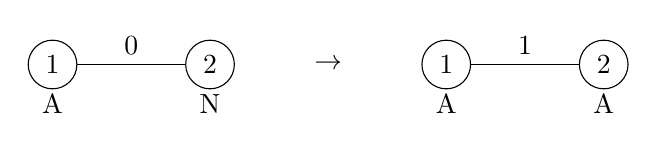
\begin{tikzpicture}
      % Left side
      \node[circle, draw] (A1) at (0,0) {1};
      \node[circle, draw] (N1) at (2,0) {2};
      \draw (A1) -- (N1) node[midway, above] {0};
      \node at (0,-0.5) {A};
      \node at (2,-0.5) {N};
  
      % Arrow
      \node at (3.5, 0) {$\rightarrow$};
  
      % Right side
      \node[circle, draw] (A2) at (5,0) {1};
      \node[circle, draw] (A3) at (7,0) {2};
      \draw (A2) -- (A3) node[midway, above] {1};
      \node at (5,-0.5) {A};
      \node at (7,-0.5) {A};
  \end{tikzpicture}
  \end{center}

  Let \( (G, \lambda) \) be a labeled graph such that all nodes are labeled \(N\) except for one node labeled \(A\), and all edges are labeled \(0\). 
  If we apply the rule \(r\) while it is possible, we obtain a labeled graph \( (G', \lambda') \) with all nodes labeled by \(A\) and all edges labeled by \(1\). Edges labeled by \(1\) in \( (G', \lambda') \) form a spanning tree of \( G \). 
\end{example}

